
\chapter{Architecture globale}
% rappeler les différents blocks SysML identifié

Ce chapitre est une description succincte de la modélisation statique du système faite dans \cite{OBCdS}.
La figure \ref{TopBDD} ci-dessous montre l'architecture matérielle et logicielle du système global, elle suit le formalisme SysML.

\begin{figure}[H]
	\centerline{
		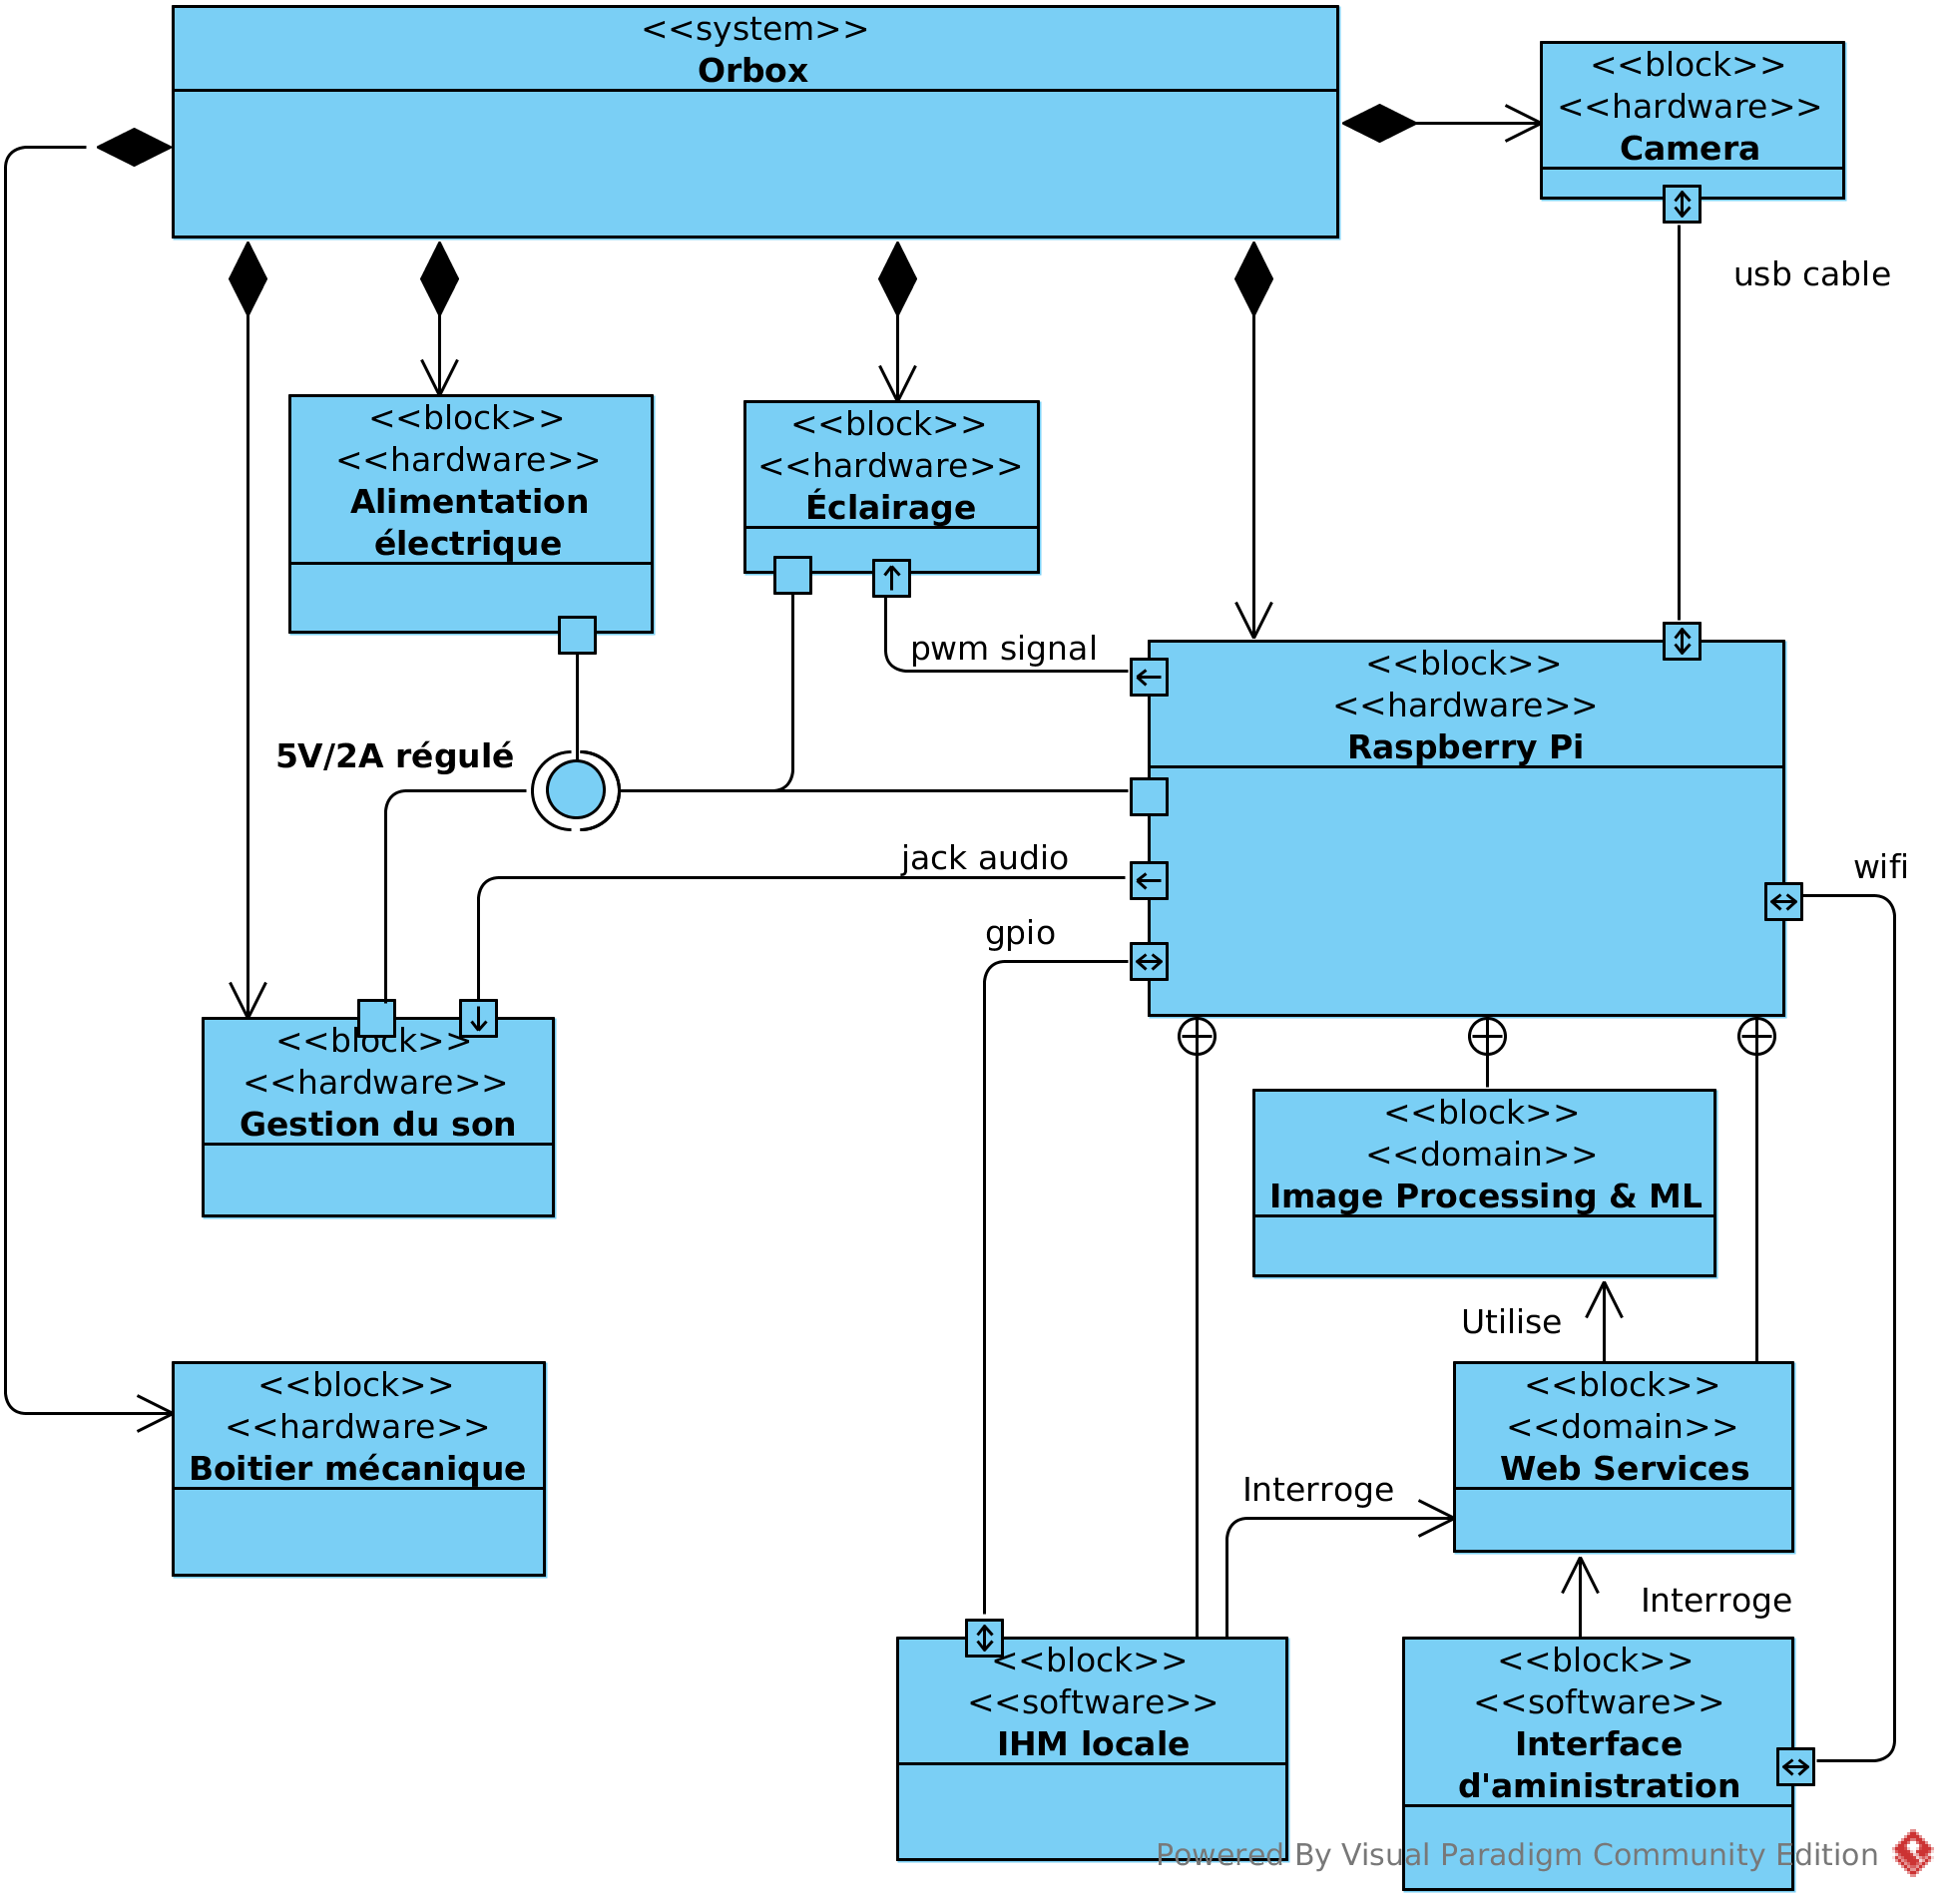
\includegraphics[scale=0.75,fbox]{img/SysML_Top_BDD.png}
	}
	\caption{Top level Block Definition Diagram}
	\label{TopBDD}
\end{figure}

Une description détaillée des composants est fournie ci-dessous :
\begin{labeling}[~--]{Interface d'administration}
	\item [Alimentation électrique] Elle a pour rôle de fournir l'énergie de manière suffisante et appropriée aux composants électroniques de la Or-Box.
	\item [Boitier mécanique] Il sert à maintenir les différents composants matériels ensemble.
	\item [Gestion du son] Elle permet de transformer et d'adapter le signal électrique en signal sonore pour la synthèse vocale.
	\item [Éclairage] Il permet d'avoir des clichés des objets posés sur la vitre malgré le contre-jour créé par la lumière ambiante.
	\item [Caméra] Elle est équipée d'un objectif fish-eye de 170 \degree d'angle de vue afin de voir toute la surface vitrée tout en maintenant un design compact.
	\item [Raspberry Pi] C'est l'ordinateur monocarte embarqué dans le système sur lequel est exécute l'ensemble des composants logiciels.
	\item [Interface d'administration] Application déportée de la Or-Box qui permet d'enrichir la base d'objet connu.
	\item [IHM Locale] Le composant logiciel qui a pour but d'orchestrer les scénarios de la Or-Box quand elle utilisé de manière autonome.
	\item [Web Services] Ils permettent l'accès à des ressources qui devront être accédées par l'interface distante d'administration et par l'IHM locale.
	\item [Image Processing \& ML]  Ce bloc logiciel contient le coeur de métier de l'application, voir le chapitre \ref{AnaLog} pour plus de détails.
\end{labeling}

